\begin{figure}[tbp]
\centering
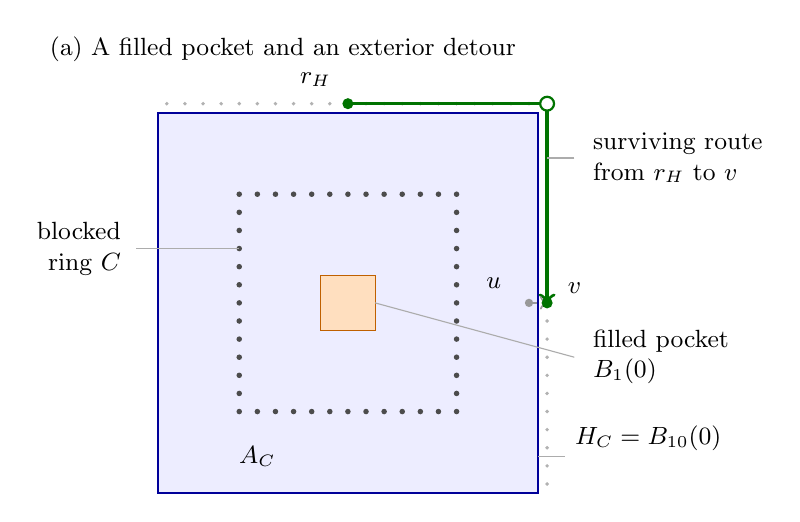
\begin{tikzpicture}[x=.23cm,y=.23cm,font=\small]
  \node[anchor=west] at (-17,14)
    {(a) A filled pocket and an exterior detour};
  \fill[blue!7] (-10.5,-10.5) rectangle (10.5,10.5);
  \draw[blue!60!black,thick] (-10.5,-10.5) rectangle (10.5,10.5);
  \fill[orange!25] (-1.5,-1.5) rectangle (1.5,1.5);
  \draw[orange!75!black] (-1.5,-1.5) rectangle (1.5,1.5);
  \foreach \n in {-6,...,6} {
    \fill[black!70] (\n,6) circle (1pt);
    \fill[black!70] (\n,-6) circle (1pt);
  }
  \foreach \n in {-5,...,5} {
    \fill[black!70] (6,\n) circle (1pt);
    \fill[black!70] (-6,\n) circle (1pt);
  }
  \foreach \n in {-10,...,10} {
    \fill[gray!60] (\n,11) circle (.7pt);
    \fill[gray!60] (11,\n) circle (.7pt);
  }
  \draw[->,green!45!black,very thick] (0,11)--(11,11)--(11,0);
  \draw[->,gray!80,dashed,thick] (10,0)--(11,0);
  \fill[green!45!black] (0,11) circle (2pt);
  \fill[green!45!black] (11,0) circle (2pt);
  \fill[gray!80] (10,0) circle (1.5pt);
  \filldraw[fill=white,draw=green!45!black,thick] (11,11) circle (2.5pt);
  \node[anchor=south east] at (-.4,11.4) {$r_H$};
  \node[anchor=east] at (9,1.1) {$u$};
  \node[anchor=west] at (11.6,.8) {$v$};
  \node at (-5,-8.5) {$A_C$};
  \node[anchor=west] at (12,-7.5) {$H_C=B_{10}(0)$};
  \draw[gray!65] (12,-8.5)--(10.5,-8.5);
  \node[anchor=east,align=right] at (-12,3)
    {blocked\\ring $C$};
  \draw[gray!65] (-11.7,3)--(-6,3);
  \node[anchor=west,align=left] at (13,-3)
    {filled pocket\\$B_1(0)$};
  \draw[gray!65] (12.5,-3)--(1.5,0);
  \node[anchor=west,align=left] at (13,8)
    {surviving route\\from $r_H$ to $v$};
  \draw[gray!65] (12.5,8)--(11,8);
\end{tikzpicture}
\par\medskip
\begin{tikzpicture}[x=.55cm,y=.4cm,font=\small]
  \node[anchor=west] at (-4,5.5)
    {(b) Adjacent hulls exchange representatives};
  \fill[blue!7] (-4,-4) rectangle (4,4);
  \draw[blue!60!black,thick] (-4,-4) rectangle (4,4);
  \fill[orange!10] (5,-4) rectangle (13,4);
  \draw[orange!75!black,thick] (5,-4) rectangle (13,4);
  \draw[gray!55] (-4.5,0)--(13.5,0);
  \foreach \x in {-4,...,13} {\fill[gray!60] (\x,0) circle (1pt);}
  \fill (0,0) circle (2.5pt);
  \fill (9,0) circle (2.5pt);
  \node[above=5pt] at (0,0) {$0$};
  \node[above=5pt] at (9,0) {$9e_1$};
  \node at (0,3.1) {$H_0=[-4,4]^d$};
  \node at (9,3.1) {$H_1=9e_1+[-4,4]^d$};
  \draw[fill=white,blue!65!black,thick] (5,0) circle (3pt);
  \draw[fill=white,orange!80!black,thick] (4,0) circle (3pt);
  \node[anchor=north east] at (3.8,-.5) {$u=4e_1=r_{H_1}$};
  \node[anchor=north west] at (5.2,-.5) {$v=5e_1=r_{H_0}$};
  \draw[->,gray!80,dashed,thick] (4,1)--(5,1);
  \node[above=3pt,fill=white,inner sep=1.5pt] at (4.5,1) {original edge};
  \draw[->,blue!65!black,very thick] (5,-2.3)--(4,-2.3);
  \node[below=4pt,fill=white,inner sep=1.5pt] at (4.5,-2.3) {routed edge};
  \node[align=center] at (4.5,-5.3)
    {$\rho(u)=v,\quad\rho(v)=u$
     \\ $\operatorname{div}\1_{v\to u}=\1_{\{v\}}-\1_{\{u\}}$};
\end{tikzpicture}
\caption{Replacing lattice edges by surviving paths.
In (a), a two-dimensional example, $C=\{z:|z|_\infty=6\}$ is a blocked
ring.  Its radius-four thickening is
$A_C=\{z:2\le|z|_\infty\le10\}$; filling the surviving pocket
$B_1(0)$ gives $H_C=B_{10}(0)$.  The original edge $u\to v$, with
$u=(10,0)$ and $v=(11,0)$, is replaced by the indicated path from
$r_H=(0,11)$ to $v$.  The open corner is a surviving interpolation
vertex outside $S_C$: a nearest-neighbor route need not remain in $S_C$
itself.  In (b), the only blocked sites are $0$ and $9e_1$.
Their filled radius-four hulls are the two
displayed lattice cubes, shown schematically in a coordinate slice; the
transverse scale is compressed.  Both $u=4e_1$ and $v=5e_1$ survive.
Choosing $r_{H_0}=v$ and $r_{H_1}=u$ sends the oriented original edge
$u\to v$ to the reverse edge $v\to u$.  This is the case of
\eqref{eq:adjacent-hull-route} in which the two boundary portions are
empty.  Applying $\rho$ again would undo this required image exchange.
Panel (a) illustrates the definitions in $d=2$; the hull and boundary
properties in every $d\ge2$ are proved in Lemma~\ref{lem:hulls}.}
\label{fig:hull-routing}
\end{figure}
